 \section{Marco Teorico} 

\begin{enumerate}[1.]

              \item ¿Qu\'e es Qlink Sense?. \\
               \\
                     \begin{center}
                    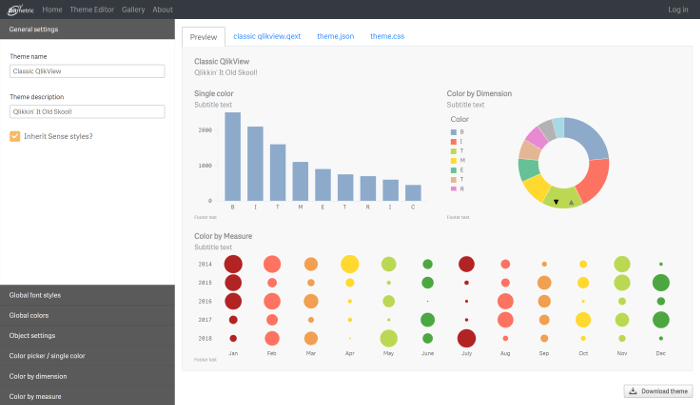
\includegraphics[scale=0.60]{./Imagenes/qlik_sense.png}
                    \end{center}
                
                   Qlik Sense es una aplicaci\'on de visualizaci\'on y descubrimiento de datos gobernada, basada en servidor, ideal para las necesidades anal\'iticas de grupos, departmentos o toda una organizaci\'on. Los usuarios de negocio obtienen un an\'alisis de datos potente, flexible y personalizado y colaboraci\'on en cualquier dispositivo, a la vez que se adhieren a unas pol\'iticas de gobierno y seguridad centralizada de datos.\\
                  \\  
              \item ¿Como podemos hacer?\\
               \\ 
               La mayor\'ia de productos de Business Intelligence (BI) ayudan a las personas a responder preguntas que ya se comprenden de antemano. Pero ¿qu\'e ocurre con las preguntas que se nos van ocurriendo despu\'es o sobre la marcha? ¿Ese tipo de preguntas que surgen tras leer un informe o visualizar un grafico? Con la experiencia asociativa de Qlik Sense, podemos hacer todas las preguntas que se nos ocurran y responderlas una tras otra, avanzando por nuestra propia ruta hacia el conocimiento. Con Qlik Sense podemos explorar los datos libremente, mediante simples clics de rat\'on, aprendiendo y profundizando en cada etapa del camino y descubriendo nuevas rutas de exploraci\'on basadas en nuestros propios descubrimientos.
              \\
              \\
               \\
               \\
              \item Utilidades \\
            \\
A trav\'es de visualizaciones inteligentes puedes: \\
             
                \begin{center}
                    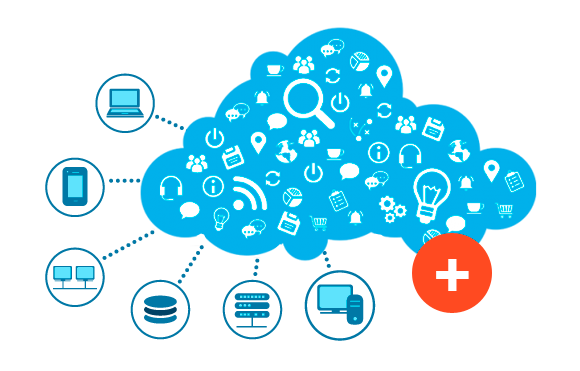
\includegraphics[scale=0.60]{./Imagenes/caracteristicas.png}
                 \end{center}

        \begin{itemize}
         \item Transmitir el significado de los datos con visualizaciones inteligentes, innovadoras, completamente interactivas y con capacidad de reacci\'on.\\
         \item Explorar en cualqxuier direcci\'on: encuentrar datos e informaci\'on valiosa que las herramientas jerarquicas y basadas en consultas no detectan.\\
         \item Lograr una flexibilidad absoluta: solo tienes que escribir lo que necesites para encontrar información relacionada y ver datos relacionados en todo el conjunto de datos.\\
          \item Explorar m\'ultiples fuentes de datos: conectar y visualizar datos de varias fuentes para una vista m\'as exhaustiva.\\
          \item Narraci\'on de datos detallada: colaborar y compartir la informaci\'on extraida del an\'alisis visual. Comunicar mejor los hallazgos a su equipo. Moverte directamente entre historias y an\'alisis en directo para responder a preguntas y acelerar la toma de decisiones.\\
        \end{itemize}

         \item  Caracteristicas 
    
       \begin{description}
            \item[Multifuente:] Se conecta con m\'ultiples fuentes de datos, incluyendo entradas de datos en tiempo real, a fin de proporcionar unas vistas aun m\'as exhaustivas, sin comprometer el rendimiento de las aplicaciones.\\
            \item[Colaborativo:] La funcionalidad de Qlik Sense le permitir\'a una narraci\'on de datos facil con la que podra compartir el análisis de una forma visual, comunicar sus hallazgos a los equipos y colaborar con mayor eficacia.\\
            \item[AutoServicio:] Cualquier usuario puede crear sus propias visualizaciones de datos, sus cuadros de mando, al tiempo que ofrece a TI la confianza de estar diseñando unas librerías seguras y consistentes y unos datos bien gobernados.\\
            \item[DragandDrop:] Las visualizaciones inteligentes, en combinaci\'on con los datos Qlik patentados de su motor de indexaci\'on, descubren todas las relaciones entre las dimensiones de datos, revelando conocimientos que habr\'ian permanecido ocultos en los modelos tradicionales de datos basados en consultas y jerarqu\'ias. Datos, informacion y conocimiento.\\

        \end{description}
               


    
\end{enumerate}
